%05/03 - Myriam
\part{Docking y dinámica molecular}
\chapter{Docking molecular}
El docking molecular es una técnica computacional con aplicaciones clave en el descubrimiento de fármacos y la química de productos naturales. Esta técnica se complementa con áreas como la quimioinformática, el cribado virtual (virtual screening) y los métodos QSAR (Quantitative Structure-Activity Relationship), que permiten predecir propiedades físicas y químicas de moléculas.

El docking molecular se aplica en cuatro bloques principales dentro del desarrollo de fármacos:
\begin{itemize}
\item \textbf{Química Combinatoria y High-Throughput Screening (HTS):} no se conoce la estructura de la proteína ni del ligando. Se generan bibliotecas de compuestos y modelos 3D de la proteína para identificar posibles ligandos.

\item \textbf{Diseño \textit{de novo}}: se conoce la estructura de la proteína, pero no la del ligando. Se estudia la cavidad de unión para identificar los aminoácidos clave y diseñar ligandos específicos. 

\item \textbf{Diseño basado en la estructura del receptor}: se conocen tanto la estructura de la proteína como la de los ligandos. El objetivo es estudiar la interacción entre ambos para optimizar la unión.

\item \textbf{Similitud del farmacóforo}: se conoce la estructura de los ligandos, pero no la de la proteína. Se utiliza un modelo de farmacóforo (patrón de características moleculares) para comparar con ligandos similares en bases de datos preexistentes.
\end{itemize}

Para realizar docking molecular, es crucial conocer la estructura de las proteínas. Las técnicas experimentales más utilizadas son:
\begin{itemize}
\item \textbf{Purificación de proteínas}: Aislamiento de la proteína de interés.
\item \textbf{Cristalografía de rayos X}: Determina la estructura atómica de la proteína en estado cristalino.
\item \textbf{Resonancia Magnética Nuclear (RMN):} Útil para proteínas en solución.
\end{itemize}

Muchas proteínas están asociadas a enfermedades, por lo que el diseño de fármacos que las inhiban o modulen puede ser clave para el tratamiento de patologías.

\section{Screening y reposicionamiento de fármacos}
El \textbf{cribado virtual} (virtual screening) es una estrategia fundamental en el descubrimiento de fármacos. Consiste en crear una \textbf{quimioteca} (colección de compuestos químicos) que se evalúa frente a proteínas de interés. Las herramientas \textbf{ADMET} (Absorción, Distribución, Metabolismo, Excreción y Toxicidad) permiten predecir si un compuesto es adecuado para estudios posteriores.
El proceso general incluye:
\begin{enumerate}
\item \textbf{Cribado virtual:} identificación de compuestos candidatos.
\item \textbf{Docking molecular:} estudio de la interacción entre los compuestos y la proteína.
\item \textbf{Dinámica molecular:} simulación del comportamiento del complejo proteína-ligando en el tiempo.
\item \textbf{Métodos de Poisson-Boltzmann:} análisis detallado de las interacciones electrostáticas.
\end{enumerate}
Finalmente, los compuestos más prometedores se validan experimentalmente mediante ensayos \textit{in vitro}.

\section{Docking molecular}
El docking molecular es una técnica computacional que predice la interacción entre una proteína y un ligando. Por ejemplo, en enfermedades neurodegenerativas, se estudian proteínas como Orai1 para identificar ligandos que modulen su actividad.

Se debe saber si hay un ligando que permita activar la función de la proteína y generar una respuesta biológica. Antes de gastar un dinero en un fármaco que puede no funcionar, primero se mira computacionalmente si se puede producir actividad en cuanto a interacción. Se conocen las conformaciones del ligando en la cavidad proteica, sabiendo previamente el sitio de interacción de la proteína y dónde se quiere ensamblar el ligando. La herramienta quizás permite descubrir otros sitios de interacción que no se conocían. 

\subsection{Tipos de docking}
Hay dos tipos de interacción o acoplamiento:
\begin{itemize}
\item \textbf{Métodos basados en ligando:} se conoce la estructura del ligando, pero no se sabe a qué proteína se puede unir. Para ello, se enfrenta y se ve con qué proteína interacciona. Se utiliza en cribado de alto rendimiento (high-throughput screening).
\item \textbf{Métodos basados en estructuras}: estos se usan principalmente para identificar las interacciones ligando-receptor, ya que se conoce la estructura de la proteína.
\end{itemize}

El docking puede considerar dos modelos. El primero es el \textbf{modelo de llave-cerradura de Fisher}, el cual considera la proteína y el ligando como estructuras rígidas. Al no poder cambiar su estructura, el objetivo es únicamente conocer si hay interacción entre ambos. El \textbf{modelo de ajuste inducido} tiene en cuenta la flexibilidad de ambas moléculas, permitiendo cambios conformacionales.

Finalmente, el docking se puede dividir en tres tipos según la flexibilidad:
\begin{itemize}
\item \textbf{Docking rígido:} tanto la proteína como el ligando se consideran rígidos, siguiendo el modelo de Fisher. Esto es útil para descartar compuestos rápidamente en caso de no haber interacción. El receptor rota y se traslada al ligando, pero no hay movimiento dentro de las estructuras durante el cálculo.
\item \textbf{Docking semiflexible:} el ligando es flexible, pero la proteína es rígida. Herramientas como AutoDock permiten este tipo de análisis. Este docking es bastante exhaustivo y permite conocer la conformación ideal del ligando. Es el que más se usa al poder usarse a nivel de usuario.
\item \textbf{Docking flexible:} tanto la proteína como el ligando son flexibles. La precisión es muy buena, pero el tiempo de cálculo es muy amplio y es necesario ejecutarlo en un clúster. Al seleccionar la zona de interacción, estos residuos son los que se definen como flexibles, no es toda la proteína. 
\end{itemize}

\subsection{Información estructural del sitio activo}
Hay dos tipos de enfoque del docking molecular: 
\begin{itemize}
\item \textbf{Acoplamiento a ciegas:} no se conoce el sitio de unión o si hay interacción entre el ligando y la proteína. Programas como Discovery Studio identifican cavidades potenciales para realizar estudios más focalizados.
\item \textbf{Acoplamiento específico:} se conoce el sitio de unión y se centra el estudio en esa región.
\end{itemize}

\section{Metodologías del docking}
Existen dos enfoques principales en docking: los métodos sistemáticos y los estocásticos. Autodock emplea principalmente métodos sistemáticos, aunque en sus versiones más recientes ha incorporado enfoques estocásticos.

En los \textbf{métodos sistemáticos}, se exploran todas las conformaciones posibles del ligando, ajustándolo hasta que encaje en la proteína. Este proceso involucra la rotación en todos los ángulos posibles, lo que lo hace menos eficiente para sistemas grandes. Por otro lado, los \textbf{métodos estocásticos} funcionan de manera opuesta: generan conformaciones aleatorias del ligando en la proteína para encontrar mínimos locales y globales de energía. Estos métodos son más adecuados para espacios explorables grandes, mientras que los sistemáticos resultan más exhaustivos y se recomiendan para estructuras pequeñas.

La formación de un complejo proteína-ligando es un proceso termodinámico que tiende hacia un equilibrio, alcanzando una energía de unión libre estable y baja. Cuando esto ocurre, el ligando se encuentra en una configuración energéticamente favorable dentro de la cavidad proteica. Para estimar estas energías de unión, se emplean diversos algoritmos matemáticos.

\subsection{Algoritmo de búsqueda}
Los algoritmos de búsqueda utilizados en docking incluyen:

\begin{itemize}
\item \textbf{Búsqueda exhaustiva}: Explora todas las conformaciones posibles del ligando (que puede ser otra proteína) y la proteína receptora, evaluando los rotámeros más favorables.

\item \textbf{Algoritmo por fragmentación}: Divide el ligando en fragmentos e inserta cada uno en la cavidad proteica de manera secuencial. Cada fragmento se optimiza antes de añadir el siguiente, construyendo progresivamente la estructura final.

\item \textbf{Monte Carlo (MC)}: Es un método estocástico que modifica aleatoriamente los grados de libertad del sistema. Evalúa la energía de interacción entre el ligando y la proteína, y si se encuentra una configuración con menor energía, se acepta. Si la energía no mejora, el programa reinicia el proceso.

\item \textbf{Algoritmo genético}: Basado en principios de evolución y selección natural, trata los grados de libertad del ligando como genes y las conformaciones finales como cromosomas. El algoritmo introduce mutaciones (cambios de conformación) y selecciona aquellas que mejoran la afinidad de unión, descartando las menos favorables.
\end{itemize}

A modo de resumen hasta ahora: tenemos la proteína y el ligando y se forma el complejo. Hay que elegir el programa más adecuado para lo que se quiere encontrar. Una vez que tenemos el cálculo hecho, hay que buscar la función de puntuación que calcula la energía de afinidad obtenida.

\section{Puntuación}
El docking genera millones de estructuras potenciales, por lo que es crucial clasificarlas según su calidad. Para ello, los programas emplean funciones de \textbf{puntuación}, que estiman, pero no calculan directamente, la energía de afinidad. Estas funciones pueden basarse en:
\begin{itemize}
\item \textbf{Campos de fuerza}: Evalúan las interacciones entre los átomos del ligando y el receptor utilizando parámetros predefinidos para describir interacciones de Van der Waals y electrostáticas.

\item \textbf{Datos empíricos}: Se basan en observaciones experimentales y en parámetros ajustados estadísticamente, incorporando factores como enlaces de hidrógeno, solvatación e hidrofobicidad.

\item \textbf{Conocimiento estructural}: Utilizan datos experimentales y literatura científica para modelar interacciones, asumiendo que los contactos más frecuentes corresponden a interacciones más favorables.
\end{itemize}

\section{Bases de datos y software}
Las principales bases de datos para la búsqueda de fármacos incluyen PubChem, ChEMBL, DrugBank y SINC.

Entre los programas de docking destacan:
\begin{itemize}
\item \textbf{Schrödinger}: Realiza docking dirigido a un sitio de unión conocido (no ciego) y permite análisis adicionales como dinámica molecular.
\item \textbf{MOE}: Permite realizar estudios QSAR (Quantitative Structure-Activity Relationship).
\end{itemize}

Las principales bases de datos de proteínas son PDB y AlphaFold. Para modelado de proteínas, se pueden utilizar:
\begin{itemize}
\item \textbf{I-TASSER}
\item \textbf{Swiss-Model}
\item \textbf{AlphaFold}
\end{itemize}

\begin{table}[h]
\centering
\begin{tabular}{l l}
Situación & Software reocmendado \\ \hline
Proteína con homólogos en PDB & Swiss-Model o I-Tasser \\
Proteína sin estructura previa & AlphaFold \\
Predicciones rápidas y sencillas & Swiss-Model \\
Predicciones detalladas y refinadas & I-TASSER \\
Acceso a GPUs y predicciones muy precisas & AlphaFold
\end{tabular}
\end{table}

\section{Esquema general de trabajo}
El proceso de docking comienza con los archivos PDB del receptor y el ligando. Estos se convierten en archivos PDBQT, que incluyen coordenadas, cargas parciales y tipos de átomos. Posteriormente, se ajusta la región de interés dentro de la proteína mediante la definición de un grid, delimitando el área donde se realizará el docking.

\begin{figure}[h]
\centering
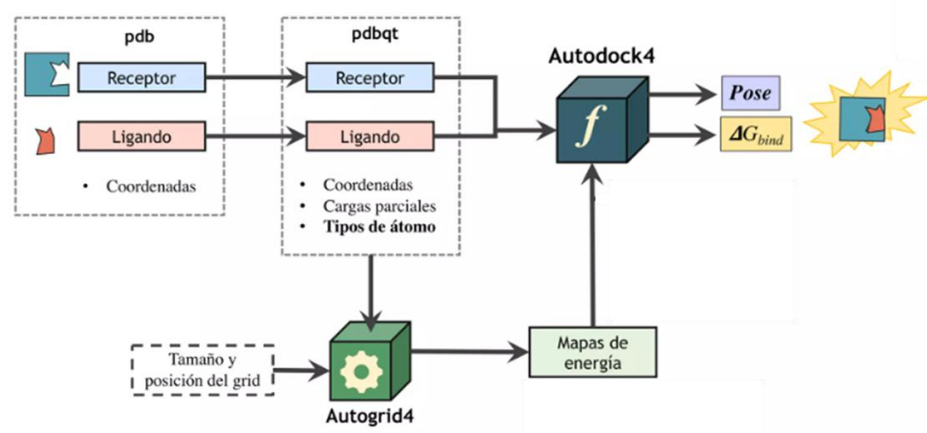
\includegraphics[width = 0.7\textwidth]{figs/docking-pipeline.png}
\end{figure}

\section{Práctica}
El ligando es el fichero jnj.pdb, y la proteína es P2X7-SWISSMODEL.pdb. Con esto localizado, vamos al programa Avogadro. Al descargar un ligando o fármaco, no es real, es plano. Por ello, Avogadro permite minimizar la estructura a una más real. 

Al final hemos utilizado la tolcapona. En PubChem hemos buscado tolcapone y descargado la estructura 3D en SDF. Esto lo abrimos en Avogadro. En la barra superior hay un botón con una E y una flecha hacia abajo (tres botones a la izquierda de Tool Settings). Seleccionamos el campo de fuerza MMFF94 con 4 pasos por update y pulsamos start. 

\begin{figure}[h]
\centering
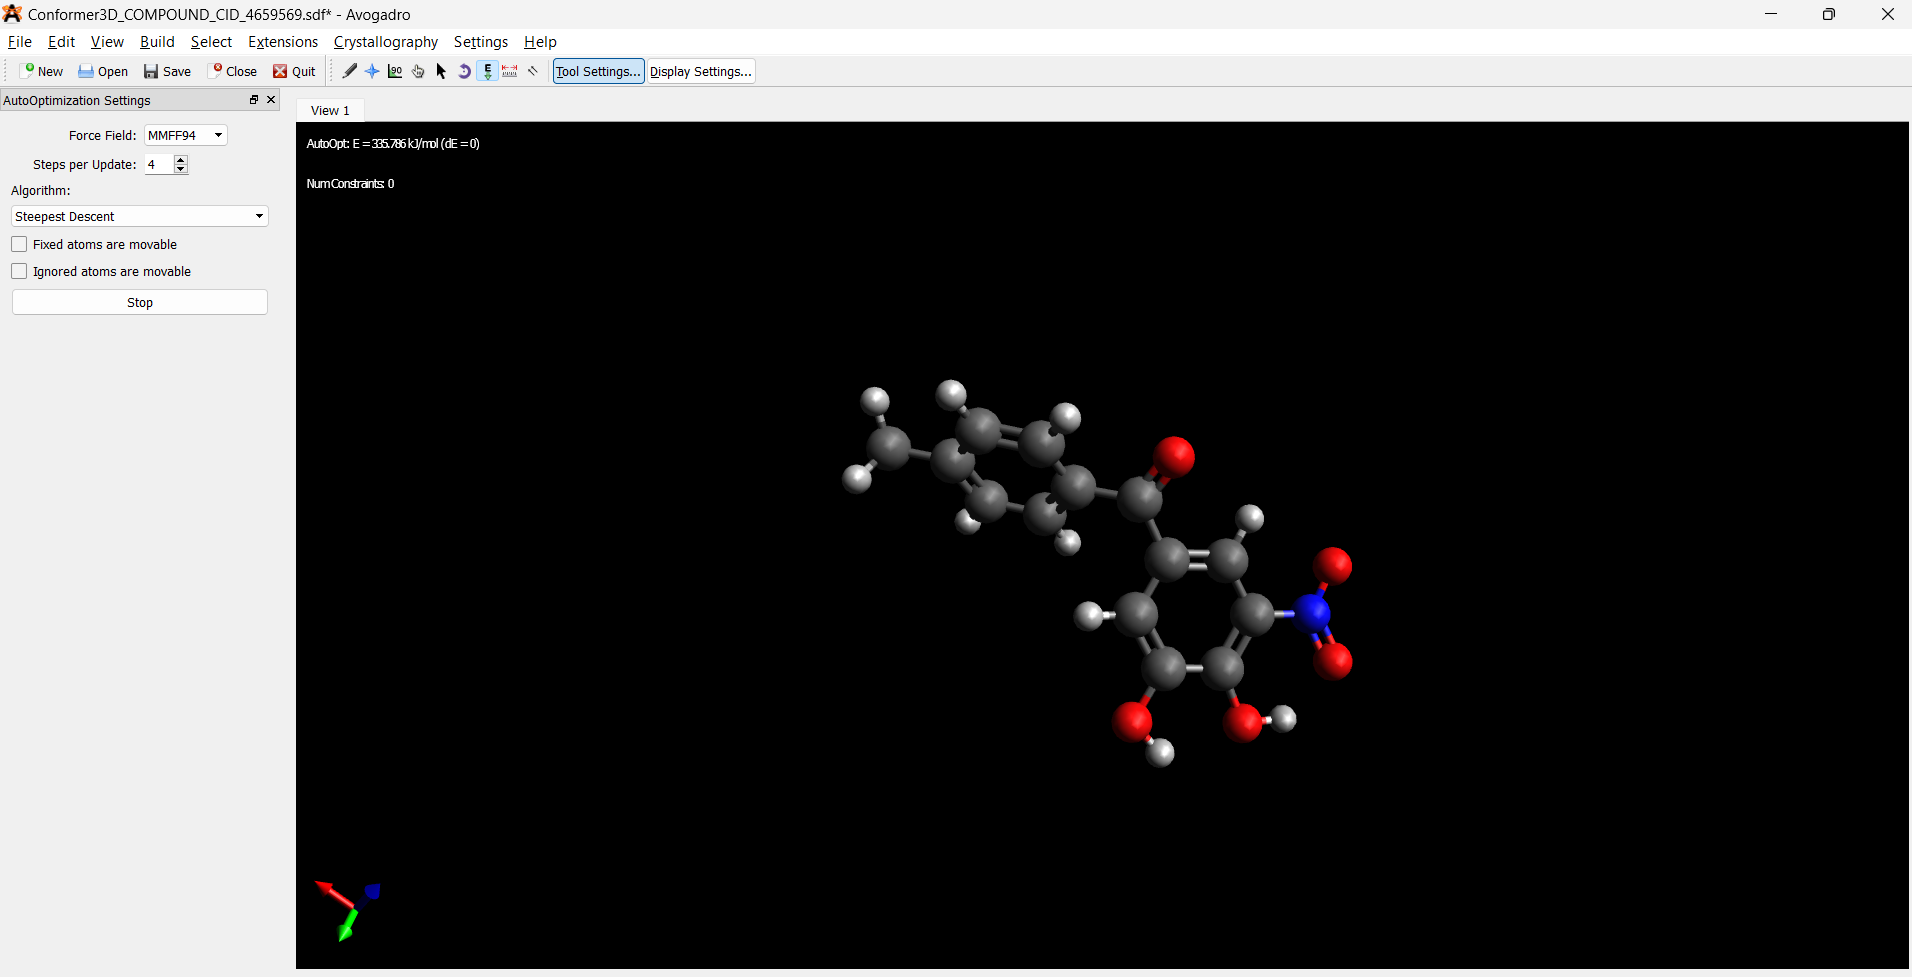
\includegraphics[width = 0.7\textwidth]{figs/avogadro-tolcapona.png}
\end{figure}

Una vez terminado, lo guardamos en formato PDB y abrimos Chimera. Ahí abrimos P2X7-Swissmodel.pdb. A continuación vamos a Tools > Surface/Binding Analysis > Dock Prep. Es importante que esté marcada la opción de "Add hydrogens" y "Add charges". Este programa trabaja con estructuras en formato Mol2 para docking, por lo que esa opción también debe estar habilitada. En la siguiente pantalla debe considerar todos los enlaces de hidrógeno. Como la histidina es el aminoácido más complejo de protonar in silico, se especifica (lo dejamos por defecto, pero en estudios in silico es importante revisarlo). En cuanto a las cargas, utilizamos los residuos estándar AMBER ff14SB. La siguiente pestaña es para guardar el archivo. Le ponemos un nombre (que en este caso es p2x7\_dockprep) y lo guardamos.

En una nueva sesión abrimos jnj y volvemos a ir a Dock Prep. Repetimos lo mismo, pero en el campo de fuerzas cambiamos AM1-BCC por Gasteiger. Vemos que la carga neta es +1 y volvemos a asegurarnos de que el método sea Gasteiger. Guardamos el ligando en formato mol2. 

Cerramos la sesión y abrimos los dos ficheros .mol2 que acabamos de generar. Debemos alejarnos, ya que las dos estructuras no están juntas. Habiendo leído bibliografía previa, sabemos que el ligando se une a la proteína en la zona de beta láminas y no en las hélices alfa. Nos interesa que el ligando se una en el centro del poro o en alguna zona lateral. Ahora vamos a Favorite > Model Panel y se desmarca la proteína para poder mover el ligando. Ahora lo podemos colocar cerca del poro. Una vez terminado, Tools > Surface/Binding Analysis > Autodock Vina > Browse y ponemos un nombre de fichero. Después de aceptar seleccionamos como receptor la proteína y ligando nuestro ligando. En Receptor search volume options ponemos un 10 en todas las filas para que aparezca la caja en cualquier sitio. Al pulsar la ruedecita del centro del ratón, se selecciona toda la proteína directamente. También podemos mover la caja independientemente y ajustarla manualmente. Idealmente, la parte de las hélices alfa está fuera. Si siempre trabajamos con la misma proteína, conviene apuntarnos las coordenadas buenas que se han actualizado en el panel anterior. En opciones de receptor deben estar todos en verdadero salvo "ignore all non-standard residues", que debe estar en falso. El resto lo dejamos por defecto salvo Number of Binding Models, que lo subimos a 10. En executable location, debemos asegurarnos de que esté el path del ejecutable (que suele estar en C:/Program Files(x86)/The Scripp Research Institute/Vina/vina.exe).

\begin{figure}[h]
\centering
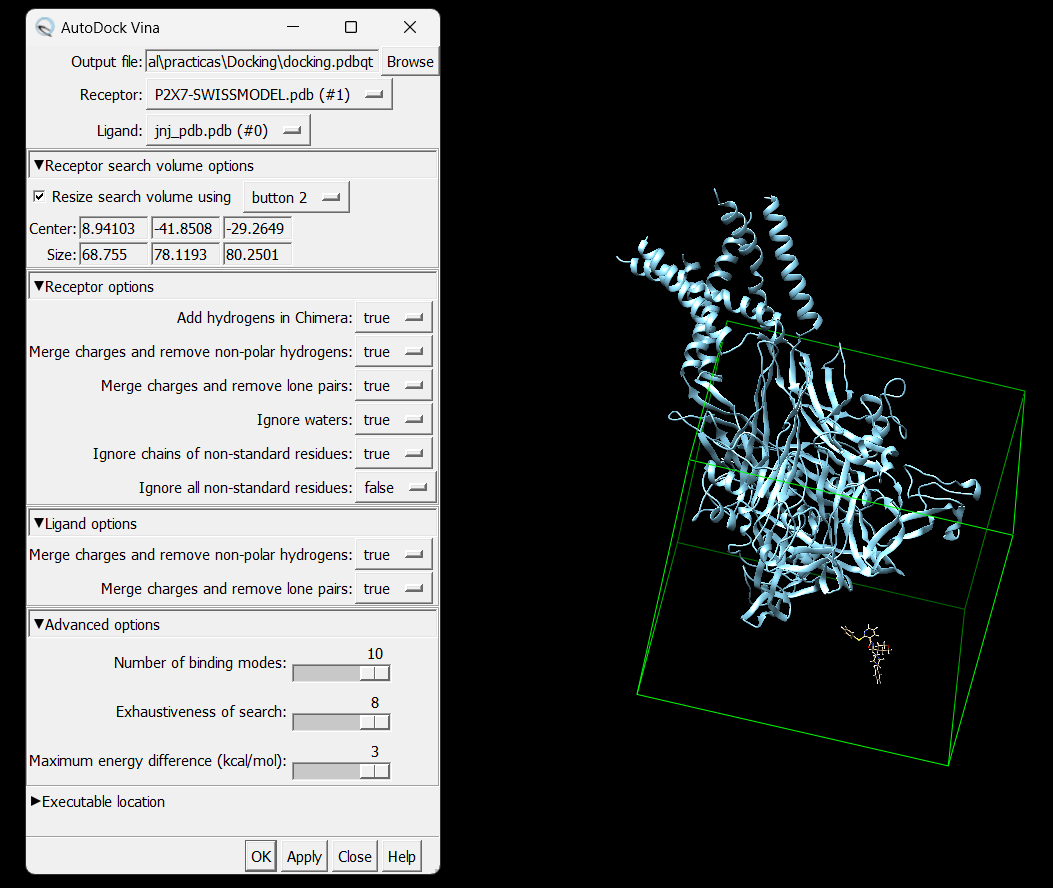
\includegraphics[width = 0.7\textwidth]{figs/docking.png}
\end{figure}

Una vez terminado, aparece una tabla con las distintas uniones ordenadas. Las interacciones deberían estar a no más de 5 $\AA$ y se debe revisar manualmente que el docking es real y no esté en mitad de la proteína. Se puede mirar en PyMOL abriendo los ficheros docking.pdbqt y docking.receptor.pdbqt. 